\documentclass{article}
\usepackage{tikz}
\usetikzlibrary{arrows.meta, positioning, shapes.multipart, calc}

\begin{document}

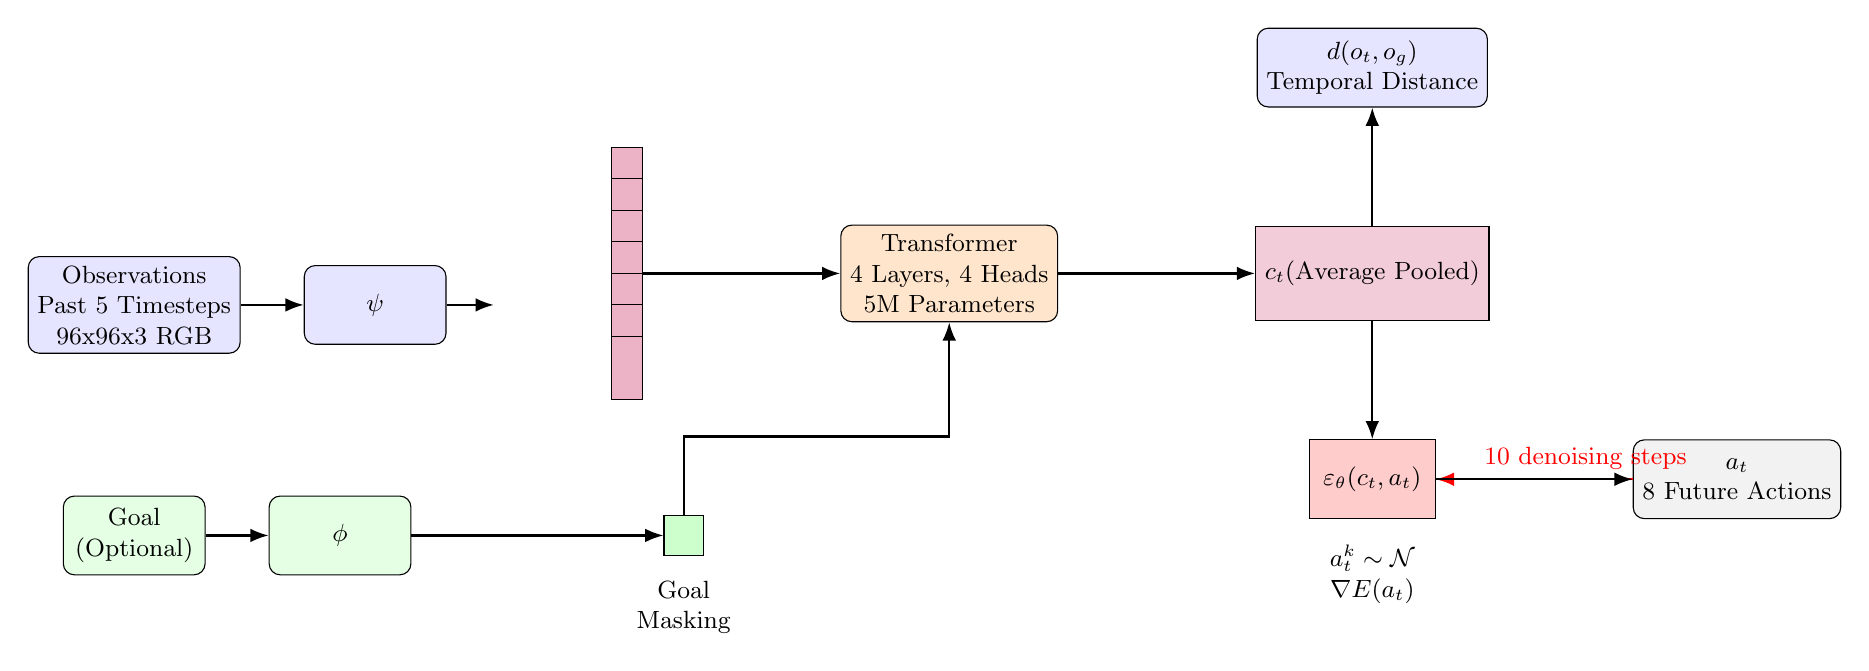
\begin{tikzpicture}[
    font=\small,
    box/.style={draw, rounded corners, align=center, minimum width=1.8cm, minimum height=1cm},
    arrow/.style={-Latex, thick},
    token/.style={rectangle, draw, fill=purple!30, minimum width=0.4cm, minimum height=0.8cm},
    goal/.style={rectangle, draw, fill=green!20, minimum width=0.5cm, minimum height=0.5cm},
    roundbox/.style={draw, rounded corners, align=center, minimum width=2.6cm, minimum height=1.2cm, fill=orange!20},
    action/.style={rectangle, draw, fill=red!20, minimum width=1.6cm, minimum height=1cm},
    context/.style={rectangle, draw, fill=purple!20, minimum width=1.6cm, minimum height=1.2cm}
]

% Observation stack
\node[box, fill=blue!10] (obs) {Observations\\Past 5 Timesteps\\96x96x3 RGB};
\node[box, fill=blue!10, right=0.8cm of obs] (psi) {$\psi$};

% Goal path
\node[box, fill=green!10, below=1.8cm of obs] (goal) {Goal\\(Optional)};
\node[box, fill=green!10, right=0.8cm of goal] (phi) {$\phi$};

% Tokens
\node at ($(psi)+(3.2,1.6)$) (token1) [token] {};
\node at ($(psi)+(3.2,1.2)$) (token2) [token] {};
\node at ($(psi)+(3.2,0.8)$) (token3) [token] {};
\node at ($(psi)+(3.2,0.4)$) (token4) [token] {};
\node at ($(psi)+(3.2,0.0)$) (token5) [token] {};
\node at ($(psi)+(3.2,-0.4)$) (token6) [token] {};
\node at ($(psi)+(3.2,-0.8)$) (token7) [token] {};

% Goal masking indicator
\node[goal, right=3.2cm of phi] (goal_token) {};

\node[align=center, below=0.2cm of goal_token] (mask_text) {Goal\\Masking};

% Transformer
\node[roundbox, right=2.5cm of token4] (transformer) {Transformer\\4 Layers, 4 Heads\\5M Parameters};

% Context
\node[context, right=2.5cm of transformer] (context) {$c_t$\\(Average Pooled)};

% Temporal Distance
\node[box, fill=blue!10, above=1.5cm of context] (dist) {$d(o_t, o_g)$\\Temporal Distance};

% Diffusion block
\node[action, below=1.5cm of context] (diffusion) {$\varepsilon_\theta(c_t, a_t)$};

% Output actions
\node[box, fill=black!5, right=2.5cm of diffusion] (actions) {\textbf{$a_t$}\\8 Future Actions};

% Denoising arrow
\draw[arrow, red, thick] (actions.west) -- ++(-1.2,0) node[midway, above] {10 denoising steps} |- (diffusion.east);

% Arrows
\draw[arrow] (obs) -- (psi);
\draw[arrow] (psi.east) -- ++(0.6,0);
\draw[arrow] (goal) -- (phi);
\draw[arrow] (phi.east) -- (goal_token.west);
\draw[arrow] (token4.east) -- (transformer.west);
\draw[arrow] (goal_token.north) -- ++(0,1.0) -| (transformer.south);
\draw[arrow] (transformer.east) -- (context.west);
\draw[arrow] (context.north) -- (dist.south);
\draw[arrow] (context.south) -- (diffusion.north);
\draw[arrow] (diffusion.east) -- (actions.west);

% Noise & Gradient labels
\node[align=center, below=0.2cm of diffusion] {$a^k_t \sim \mathcal{N}$\\$\nabla E(a_t)$};

\end{tikzpicture}

\end{document}
